\documentclass[journal]{IEEEtran}
\usepackage{balance}
\usepackage{color}
\usepackage{float}
\usepackage{amssymb}
\usepackage{cite}
\usepackage{amsmath}
\usepackage{amsthm}
\newtheorem{Lemma}{Lemma}
\newtheorem{corollary}{Corollary}
\renewcommand\qedsymbol{}
\usepackage{enumerate}
\usepackage{algorithm}
\usepackage{algpseudocode}
\usepackage{graphicx}
\usepackage{epstopdf}
\epstopdfsetup{outdir=./}
\graphicspath{{images/}}
\usepackage{booktabs}
\usepackage{multirow}
\usepackage{bm}
\usepackage{url}
\usepackage{tabularx}
\usepackage{placeins}
\newcommand{\revision}[1]{\textcolor{blue}{#1}}
% Marked copy: also flag revision-added structural blocks (theorems, proofs, tables) in blue.
\usepackage{etoolbox}
\AtBeginEnvironment{Lemma}{\color{blue}}
\AtBeginEnvironment{corollary}{\color{blue}}
\AtBeginEnvironment{proof}{\color{blue}}
\AtBeginEnvironment{table}{\color{blue}}
\AtBeginEnvironment{table*}{\color{blue}}
\setlength{\textfloatsep}{4pt plus 1pt minus 1pt}
\setlength{\floatsep}{4pt plus 1pt minus 1pt}
\setlength{\intextsep}{4pt plus 1pt minus 1pt}
\setlength{\abovecaptionskip}{2pt plus 1pt minus 1pt}
\setlength{\belowcaptionskip}{1pt plus 1pt minus 1pt}
\setlength{\abovedisplayskip}{2pt plus 1pt minus 1pt}
\setlength{\belowdisplayskip}{2pt plus 1pt minus 1pt}
\setlength{\abovedisplayshortskip}{1pt plus 1pt minus 1pt}
\setlength{\belowdisplayshortskip}{1pt plus 1pt minus 1pt}
\setcounter{topnumber}{5}
\setcounter{bottomnumber}{5}
\setcounter{totalnumber}{10}
\renewcommand{\topfraction}{0.95}
\renewcommand{\bottomfraction}{0.90}
\renewcommand{\textfraction}{0.05}
\renewcommand{\floatpagefraction}{0.85}
\renewcommand{\dbltopfraction}{0.95}
\renewcommand{\dblfloatpagefraction}{0.85}

% Correct bad hyphenation here
\hyphenation{op-tical net-works semi-conduc-tor}

\begin{document}

\title{MAML-Select: An Online Adaptive Client Selection Method for Federated Learning via Meta-Learning}

%\author{Aakash Sharma, Advait Pathak, Ricktho Sarkar, Om Jee Pandey, \textit{Senior Member, IEEE}
%\thanks{A. Sharma, A. Pathak, and R. Sarkar are undergraduate researchers at IIT BHU Varanasi, Varanasi 221005, India.}
%\thanks{O. J. Pandey is with the Department of Electronics Engineering, IIT BHU Varanasi, Varanasi 221005, India (e-mail: omjee.ece@iitbhu.ac.in).}}

\maketitle

% =====================================================================
% ABSTRACT
% =====================================================================
\begin{abstract}
% \revision{Federated Learning (FL) enables collaborative model training across distributed edge data, however client selection remains difficult when devices differ in data distribution, compute capacity, energy state, and communication latency. Selecting only the fastest or most statistically useful clients can slow convergence, increase resource cost, or reduce participation coverage. System-aware selectors such as FedCS and TiFL address stragglers, while utility-aware methods such as Oort, FedCor, CriticalFL, and FedGCS use loss, correlation, critical-period, or generative signals to improve training. However, many existing methods rely on fixed scoring rules, costly modelling stages, or feedback that does not explicitly adapt the selector before every round. The remaining gap is a lightweight policy that can rapidly re-rank clients as their utility and system state change dynamically during FL. We propose \textbf{Model Agnostic Meta-Learning Select (MAML-Select)}, an online adaptive selector that treats each FL round as a meta-learning task. A compact Multilayer Perceptron (MLP) is adapted with a first order update of MAML-Select from recent local-loss and latency feedback, then used to score available clients before a query-set meta-update. Across Fashion-MNIST, CIFAR-10, and CIFAR-100 with $100$ clients, $K=10$, Dirichlet $\alpha=0.5$, and three seeds, MAML-Select reduces cumulative Tera Floating-Point Operations (TFLOPs) by up to $21.5\%$ and modelled energy by up to $24.7\%$ relative to FedAvg on all three datasets, with paired-test support ($p<0.05$). Accuracy remains competitive with FedAvg and FedGCS, with the largest trade-off on CIFAR-10. These findings suggest that meta-adaptive client selection can make edge AI deployments more resource-conscious.}
\revision{In Federated Learning (FL), choosing clients for updating the shared model in each round is a combinatorial,  resource constraints, and NP-hard scheduling problem. Clients differ in data utility, training speed, battery capacity and bandwidth. Since only a small cohort can communicate per round, conventional client-selection strategies often favor clients with high training utility or fast updates, which  can repeatedly select a narrow group of clients, leaving slower or temporarily low-utility clients underused, reducing participation coverage, and making training process less efficient. Existing methods like FedCS and TiFL use system state to reduce straggler effects, whereas Oort, FedCor, CriticalFL, and FedGCS score clients using training utility, loss correlation, critical-period timing, or learned client combinations. However, these methods often rely on a fixed scoring rule, or update it slowly, even though a client’s usefulness changes as the global model evolves. \textbf{Model-Agnostic Meta-Learning Select (MAML-Select)} removes this fixed-rule assumption, and frames each round as a fast adaptation task. A lightweight policy network is learned using the previous round’s observed loss reduction and latency, and is used for ranking clients. % after one first-order MAML adaptation step using the previous round’s observed loss reduction and latency. 
After the selected clients return their updates, the same policy is meta-updated using the new feedback. We evaluate MAML-Select on Fashion-MNIST, CIFAR-10, and CIFAR-100 with 100 clients, K = 10 selected clients per round, a Dirichlet non-IID split with $\alpha=0.5$, and three random seeds. On Fashion-MNIST, CIFAR-10, and CIFAR-100, MAML-Select provides competitive accuracy with significantly lower cumulative Tera Floating-Point Operations (TFLOPs) and modelled energy consumption. Higher values of Jain-index values also demonstrates the fairness of the proposed method. %Overall, MAML-Select provides a resource-aware client-selection strategy with competitive accuracy and low client-training computational cost.
}
\end{abstract}
\renewcommand\IEEEkeywordsname{Impact Statement}
\begin{IEEEkeywords}
\revision{FL is central to privacy-preserving AI across heterogeneous environments, such as mobile health, intelligent transportation, industrial sensing, and smart-city systems, but these deployments often face tight computational-capacity, energy-consumption, and latency budgets. MAML-Select contributes an adaptive selection mechanism that reduces unnecessary client-training computational cost while preserving broad participation coverage. By using recent training feedback to re-rank clients, the method supports FL systems that respond to changing device conditions instead of relying on a fixed rule. The reported energy-consumption values are modelled estimates that follow the declared simulator and device-tier setup, giving a transparent basis for comparing selection policies. The broader impact is a more resource-aware path for deploying distributed AI at the edge, including the industrial Internet of Things (IoT), especially when model updates must remain efficient, reproducible, and privacy-preserving.}


%This enables more scalable and energy-efficient privacy-preserving AI on resource-constrained edge devices.
\end{IEEEkeywords}
\renewcommand\IEEEkeywordsname{Index Terms}
\begin{IEEEkeywords}
Federated learning, client selection, meta-learning, and computational efficiency.
\end{IEEEkeywords}
% =====================================================================
% I. INTRODUCTION
% =====================================================================
\section{Introduction}

\IEEEPARstart{F}{ederated} Learning (FL) trains a shared model across many devices without moving their raw data to the server.~\cite{mcmahan2017communication}. \revision{Clients train models locally and share only model updates. However, they differ in hardware, network conditions, and local data. Their heterogeneity creates statistical drift under non-independent and identically distributed (non-IID) data and straggler delays under synchronous training}~\cite{karimireddy2020scaffold,mai2024study,tapwal2026stragglers,forootani2026asynchronous,borazjani2026redefining}. Despite these advances, the problem of \textit{whom to select} each round remains open.

Client selection chooses a subset $\revision{\mathcal{S}_t} \subset \{1, \ldots, N\}$ each round. \revision{Client utility is non-stationary: a useful client can become redundant later, while an overlooked client can become important in the long run.} System-aware methods improve client participation, however, selection bias avoids the fairness among clients as well as slow yet data-rich clients~\cite{nishio2019client,chai2020tifl}. Utility-aware methods prioritize information gain, but may incur high latency or expensive server-side modelling~\cite{lai2021oort,tang2022fedcor,xu2024federated,yan2023criticalfl,ning2024fedgcs}. Learning-based selectors use histories, features, or reinforcement signals~\cite{wang2020optimizing,pan2024contextual,kazemi2026robust}. \revision{An efficient round-by-round mechanism for adapting the ranking policy to evolving utility remains underexplored.}

\revision{We propose MAML-Select, a client-selection framework based on a Model-Agnostic Meta-Learning (MAML)-style fast adaptation step~\cite{finn2017model}, which learns the policy network via recent feedback before the next ranking decision. Unlike reinforcement-learning (RL)-based or contextual-bandit selectors, the proposed MAML-Select uses rapid gradient-based policy adaptation. Unlike personalization of FL client models}~\cite{fallah2020personalized}, \revision{the proposed MAML adapts the selector, rather than the client model. The proposed approach is useful when devices have limited computational capacity, strict deadlines, or intermittent connectivity.} The major contributions can be summarized as follows.
\begin{enumerate}
\setlength{\itemsep}{0pt}
\setlength{\topsep}{1pt}
		\item We formulate the FL client selection problem as a meta-learning task and introduce the MAML-Select algorithm with \revision{rapid gradient-based} adaptation for online client selection.
        \item \revision{Experiments on Fashion-MNIST, CIFAR-10, and CIFAR-100 under non-IID settings ($\alpha = 0.5$, three seeds) show that MAML-Select delivers accuracy competitive with FedAvg and FedGCS at lower computational cost, and higher accuracy than FedCS, Oort, TiFL, and FedCor; sensitivity and ablation studies over $\lambda$, the inner-loop steps, the selector width, and the state features support the design choices.}
		\item We demonstrate that MAML-Select \revision{\textit{lowers cumulative training TFLOPs} by up to $21.5\%$ and modelled energy consumption by up to $24.7\%$ relative to FedAvg, with paired-test support for the resource reductions}.
\end{enumerate}

\textit{Organization:} The rest of this paper is organized as follows. Section~II reviews related work on client selection in FL. Section~III details the system model and problem formulation. The proposed MAML-Select algorithm is described in Section~IV, followed by evaluation and results in Section~V. Section~VI concludes this paper and discusses future research directions.

% =====================================================================
% II. RELATED WORK
% =====================================================================
\section{Related Work}
In the following, the classification of existing client selection methods for the FL algorithm are presented. 
\subsubsection{System-Aware Selection}
System-aware selection addresses stragglers. FedCS selects feasible clients under resource constraints, while TiFL groups devices into online performance tiers~\cite{nishio2019client,chai2020tifl}. Recent studies show similar concerns for slow but data rich clients in resource-constrained medical IoT and asynchronous FL with heterogeneous objectives~\cite{tapwal2026stragglers,forootani2026asynchronous}. MAML-Select uses feedback from the previous training phase, and learns the selection policy based on six parameters. %while learning how much they should matter in the current training phase.

\subsubsection{Data-Aware and Utility-Based Selection}
Data-aware methods select clients for model utility rather than only speed. Oort prioritizes data-rich and fast clients, and FedCor models correlations between client losses~\cite{lai2021oort,tang2022fedcor}. CriticalFL uses critical learning periods, while FedGCS searches for client combinations in a learned continuous space~\cite{yan2023criticalfl,ning2024fedgcs}. Other work couples selection with aggregated design~\cite{xu2024federated,tran2026fedimp}. MAML-Select instead targets rapid adaptation of the ranking policy as client utility evolves.

\subsubsection{Learning-Based and Meta-Learning Approaches}
Learning-based selectors improve from observed feedback. FAVOR uses a deep Q-network (DQN), while neural contextual bandits learn from client features and rewards~\cite{wang2020optimizing,pan2024contextual}. Recent work also studies deep-RL selection for robustness and fairness-aware inclusive participation~\cite{kazemi2026robust,arisdakessian2026vox}. In ~\cite{fallah2020personalized}, MAML is employed to personalize client FL models; however, in this work, MAML-Select adapts the server-side ranking policy, rather than the FL models.

\revision{Table~\ref{tab:related_work_comparison} consolidates these distinctions. For methods without a stated closed-form selection complexity, it reports the dominant server-side operation.}

\begin{table*}[!t]
    \color{blue}
    \caption{Comparison of representative methods and MAML-Select.}
    \label{tab:related_work_comparison}
    \centering
    \scriptsize
    \setlength{\tabcolsep}{3pt}
    \renewcommand{\arraystretch}{0.98}
    \begin{tabularx}{\textwidth}{lXXXX}
        \toprule
        \textbf{Method} & \textbf{Primary objective} & \textbf{Adaptation mechanism} & \textbf{Selection complexity or dominant operation} & \textbf{Optimization strategy} \\
        \midrule
        FedCS~\cite{nishio2019client} & Increase feasible updates under resource constraints & Resource estimates before selection & Resource-constrained subset search & Deadline-aware scheduling \\
        TiFL~\cite{chai2020tifl} & Mitigate stragglers while preserving accuracy & Online tier updates & Tiering and probabilistic sampling & Adaptive tier-based selection \\
        Oort~\cite{lai2021oort} & Improve time-to-accuracy & Utility and speed feedback & Utility scoring and guided sampling & Exploration and exploitation \\
        FedCor~\cite{tang2022fedcor} & Accelerate convergence under non-IID data & Loss-correlation model & Gaussian process (GP) covariance operations & GP-based active selection \\
        FAVOR~\cite{wang2020optimizing} & Counterbalance non-IID bias & Experience-driven policy updates & DQN inference and training & Deep Q-learning \\
        NCCB~\cite{pan2024contextual} & Learn contextual client combinations & Client features and reward feedback & Locality-sensitive hashing (LSH) feature extraction and bandit updates & Neural contextual combinatorial bandit \\
        FedCG~\cite{xu2024federated} & Couple selection and gradient compression & Capability-aware compression updates & Submodular optimization and linear programming & Joint iterative optimization \\
        CriticalFL~\cite{yan2023criticalfl} & Exploit critical learning periods & Period-aware participation & Base-selector dependent & Selector augmentation \\
        FedGCS~\cite{ning2024fedgcs} & Optimize client combinations & Search in a learned continuous space & Latent-space optimization and beam search & Gradient-based generative selection \\
        Kazemi et al.~\cite{kazemi2026robust} & Improve robustness under poisoning attacks & Experience-driven policy updates & Deep-RL inference and training & Deep reinforcement learning \\
        Vox Populi~\cite{arisdakessian2026vox} & Promote fair and inclusive participation & Fairness-aware client selection & Framework-dependent & Inclusive selection framework \\
        Per-FedAvg~\cite{fallah2020personalized} & Personalize the client model to local data & MAML adaptation of the client model, not the selector & No client selection; per-client model fine-tuning & Model-level meta-learning \\
        \textbf{MAML-Select} & Adapt rankings under evolving client utility & Fast adaptation from recent round feedback & $\mathcal{O}(N|\phi|)$ scoring plus a gradient-adaptation step & Gradient-based meta-learning \\
        \bottomrule
    \end{tabularx}
\end{table*}

\revision{\textbf{Difference from prior work:} MAML-Select meta-learns the selection policy $h_\phi$: unlike heuristic, RL, contextual-bandit, and generative selectors, it uses a MAML inner update to convert recent feedback into fast policy weights before the next cohort is scored. A fixed heuristic or bandit may update rewards over time, but does not adapt the scoring-network parameters from a support set immediately before selection.}

% =====================================================================
% III. SYSTEM MODEL AND PROBLEM FORMULATION
% =====================================================================
\section{System Model and Problem Formulation}
\revision{We consider a central server and $N$ heterogeneous clients indexed by $\mathcal{N} = \{1, 2, \ldots, N\}$. Client $i$ stores a local dataset $\mathcal{D}_i$ with $n_i$ samples.} The global objective is to minimize the empirical risk over the distributed data as
\begin{equation}
	\min_{\theta \in \mathbb{R}^d} F(\theta) = \sum_{i=1}^{N} \frac{n_i}{n} F_i(\theta),
	\label{eq:global_objective}
\end{equation}
\revision{where $\theta \in \mathbb{R}^d$ denotes the global model, $n = \sum_{i=1}^{N} n_i$, and $F_i(\theta) = \frac{1}{n_i} \sum_{j=1}^{n_i} \ell(\theta; x_{i,j}, y_{i,j})$ is the local empirical risk, with $\ell(\cdot)$ the per-sample loss (e.g.\ cross-entropy).}

\revision{At round $t$, let $\mathcal{A}_t \subseteq \mathcal{N}$ denote the available clients and $\mathcal{S}_t \subseteq \mathcal{A}_t$ the selected cohort. The server maintains the global model and selection policy; clients keep data local and return only model updates, loss summaries, and resource-state feedback. Selection is thus a server-side decision before each broadcast, with only a small fraction of clients training per round.}

\revision{Client $i$ has per-round latency $T_{i,t}=T_{i,t}^{comp}+T_{i,t}^{comm}$, split into computation and communication. The computation time is $T_{i,t}^{comp} = E\, n_i\, C_{model}/f_{i,t}$, where $E\, n_i\, C_{model}$ is the total local-training work over $E$ epochs and $n_i$ samples, $C_{model}$ is the per-sample computational cost (forward-plus-backward FLOPs), and $f_{i,t}$ is the device's effective processing rate in FLOPs/s, set by its hardware tier. The communication time is $T_{i,t}^{comm} = M/B_{i,t} + \delta_{i,t}$, where $M$ is the size of the uploaded model update, $B_{i,t}$ is the uplink bandwidth, and $\delta_{i,t}$ is a fixed propagation/queuing delay~\cite{nishio2019client}. %This is the standard computation-plus-communication FL latency model~\cite{nishio2019client}. 
In synchronous FL, the slowest selected client determines the round latency:}
\begin{equation}
	\color{black}
	T_t^{round} = \max_{i \in \mathcal{S}_t} T_{i,t}.
	\label{eq:round_latency}
\end{equation}


\revision{Let $a_{i,t}$ indicate whether client $i$ is selected. Under policy $\pi_\phi$, the constrained client-selection problem is}
\begin{equation}
	\color{blue}
	\begin{aligned}
		\min_{\pi_\phi}\quad & \sum_{t=1}^{T} \left[F(\theta_{t+1}) + \lambda T_t^{round}\right] \\
		\text{s.t.}\quad & \sum_{i=1}^{N} a_{i,t}=K,\quad a_{i,t}\in\{0,1\}, \\
		& a_{i,t}\leq \mathbf{1}\{i\in\mathcal{A}_t\},		
	\end{aligned}
	\label{eq:bi_objective}
\end{equation}
\revision{where $K$ is the cohort size, $T$ is the number of rounds, and $\lambda \geq 0$ controls the latency--loss trade-off, and the client selection subset is updated as $\mathcal{S}_t=\{i:a_{i,t}=1\}$. A larger $\lambda$ places more emphasis on latency, while $\lambda=0$ yields loss-only selection. We assume $|\mathcal{A}_t|\geq K$. The model $\theta_{t+1}$ results from local training and aggregation over $\mathcal{S}_t$. The problem remains challenging because the action space is combinatorial and client utility evolves during training.}

% =====================================================================
% IV. METHODOLOGY: MAML-SELECT
% =====================================================================
\section{MAML-Select Algorithm}
\revision{Building on~\eqref{eq:bi_objective}, MAML-Select treats client selection as a meta-learning problem: client utility changes as training progresses. In the following, algorithmic details of selection policy are given.}

\subsubsection{State Space}
\revision{The server constructs a state vector $\bm{s}_{i,t} \in \mathbb{R}^6$ for each client $i$ at round $t$. It contains local training loss $\hat{L}_{i,t}$, gradient norm $\|\nabla F_i\|_2$, estimated latency $\hat{T}_{i,t}$, battery level $b_{i,t}$, selection frequency $q_{i,t}$, and staleness $\tau_{i,t}$ (rounds since last selected)}~\cite{pan2024contextual,xu2024federated}. The state vector $\bm{s}_{i,t}$ has six entries: Statistical utility ($\hat{L}_{i,t}$, $\lVert\nabla F_{i}\rVert_{2}$), System feasibility ($\hat{T}_{i,t}$, $b_{i,t}$) and Participation balance ($q_{i,t}$, $\tau_{i,t}$). The local training loss $\hat{L}_{i,t}$ tells us if the client still has useful gradients. The gradient norm $\lVert\nabla F_{i}\rVert_{2}$ tells us the size and value of the update. The estimated latency $\hat{T}_{i,t}$ tells us the straggler and round-time risk. The battery level $b_{i,t}$ tells us the energy feasibility and the drop-out risk. he selection frequency $q_{i,t}$ helps avoid over-using a few clients. The staleness $\tau_{i,t}$, the rounds since last selected, helps avoid starving clients.
%\revision{Loss and gradient norm characterize statistical utility; latency and battery level, system constraints; selection frequency and staleness, participation imbalance. 
Each round $t$ is a task $\mathcal{T}_t$: rank clients so that the top-$K$ cohort minimizes the per-round utility.%}

MAML-Select trains a meta-policy network $h_\phi(\bm{s}_{i,t})$, parameterized by $\phi$, that learns an adaptable policy to the current round using data from the preceding round. \revision{The policy is a $6$-$64$-$64$-$1$ multilayer perceptron (MLP) with ReLU activations and 4,673 trainable parameters.} The support set represents the past experience: $\mathcal{D}_{sup}(t) = \{(\bm{s}_{i,t-1}, c_{i,t-1}) \mid i \in \revision{\mathcal{S}_{t-1}}\}$, containing client states and observed costs from round $t-1$. \revision{The candidate set represents the current decision: $\mathcal{D}_{cand}(t) = \{\bm{s}_{i,t} \mid i \in \mathcal{A}_t\}$, containing the states of available clients.}

\subsubsection{Utility Function}
\revision{The per-client utility $c_{i,t}$ supplies feedback to the ranking policy. Consistent with~\eqref{eq:bi_objective}, the utility of the client $i$ is defined as}
\begin{equation}
	\color{black}
	c_{i,t} = \lambda \underbrace{\max(0, T_{i,t} - T_{target})}_{\text{latency penalty}} - \underbrace{\Delta_{i,t}}_{\text{local loss reduction}},
	\label{eq:cost}
\end{equation}
\revision{where $\Delta_{i,t}=\hat{L}_{i,t}^{before}-\hat{L}_{i,t}^{after}$ is the local loss reduction for selected client $i$ ($\hat{L}_{i,t}^{before}$ before and $\hat{L}_{i,t}^{after}$ after its $E$ local epochs), thus $\Delta_{i,t}>0$ marks a useful update. %is a client-level proxy for statistical utility that needs no server-held validation set. 
The target $T_{target}$ is a soft deadline, and minimizing $c_{i,t}$ favors lower latency and larger loss reduction.}

\subsection{The MAML-Select Algorithm}
The algorithm proceeds in three phases per round:

\textbf{Phase~1 (Inner Loop Adaptation (Look-Ahead)):}
At the start of round $t$, \revision{the server adapts the meta-policy $\phi_t$ on $\mathcal{D}_{sup}(t)$ using one gradient-descent step:}
\begin{equation}
	\color{black}
		\phi'_t = \phi_t - \beta \nabla_{\phi_t} \mathcal{L}_{sup}(h_{\phi_t};\mathcal{D}_{sup}(t)),
		\label{eq:inner_loop}
\end{equation}
where $\mathcal{L}_{sup}$ is the mean-squared-error (MSE) loss between predicted scores and observed costs from round $t-1$, and $\beta$ is the inner learning rate.

{\color{black}
\begin{Lemma}[Inner-step descent]\label{stmt:inner}
Let the support loss $g_t(\phi)=\mathcal{L}_{sup}(h_\phi;\mathcal{D}_{sup}(t))$ be $L$-smooth, that is, $\nabla g_t$ is $L$-Lipschitz. If the inner step size obeys $0<\beta<2/L$, the inner update~\eqref{eq:inner_loop} is a descent step on the support loss:
\[
g_t(\phi'_t)\le g_t(\phi_t)-\beta\Bigl(1-\tfrac{L\beta}{2}\Bigr)\lVert\nabla g_t(\phi_t)\rVert_2^2 .
\]
\end{Lemma}
\begin{proof}
By $L$-smoothness, $g_t$ obeys the descent lemma
\[
g_t(\psi)\le g_t(\phi)+\nabla g_t(\phi)^{\top}(\psi-\phi)+\tfrac{L}{2}\lVert\psi-\phi\rVert_2^2 .
\]
Substituting $\psi=\phi'_t$, $\phi=\phi_t$, and the inner update $\phi'_t-\phi_t=-\beta\nabla g_t(\phi_t)$ yields the stated bound, whose coefficient $\beta(1-L\beta/2)$ is positive precisely for $0<\beta<2/L$; the step therefore never increases $g_t$ and strictly decreases it unless $\nabla g_t(\phi_t)=0$.
\end{proof}
A single support-set step therefore reduces the round's ranking loss, justifying adaptation before the current candidates are scored.
}

\textbf{Phase~2 (Client Selection):}
\revision{The adapted policy $h_{\phi'_t}$ scores the available clients and selects the $K$ clients with the lowest predicted costs:}
\begin{equation}
	\color{black}
	\mathcal{S}_t = \operatorname{Top-}K_{i \in \mathcal{A}_t} \left( -h_{\phi'_t}(\bm{s}_{i,t}) \right).
	\label{eq:selection}
\end{equation}

\textbf{Phase~3 (FL Execution and Outer Loop Update):}
\revision{The selected clients perform standard FL training. Their observed costs form $\mathcal{D}_{query}(t)=\{(\bm{s}_{i,t},c_{i,t})\mid i\in\mathcal{S}_t\}$. %The query loss is also the MSE. 
The meta-policy is updated on this query set:}
\begin{equation}
		\color{black}
		\phi_{t+1} \leftarrow \phi_t - \eta \nabla_{\phi'_t} \mathcal{L}_{query}(h_{\phi'_t}; \mathcal{D}_{query}(t)),
		\label{eq:outer_loop}
\end{equation}
\revision{where $\eta$ is the meta-learning rate. %We use a first-order MAML-style approximation: the 
Query-loss gradient is evaluated at the adapted weights $\phi'_t$ and applied to the meta-parameters $\phi_t$, which omits the second-order derivatives. The full procedure is detailed in Algorithm~\ref{alg:maml_select} and Fig.~\ref{fig:model_diagram}.}

{\color{black}
\begin{Lemma}[Outer-step descent]\label{stmt:outer}
Let the query loss $q_t(\phi)=\mathcal{L}_{query}(h_\phi;\mathcal{D}_{query}(t))$ be $L_q$-smooth, and let
\[
\delta_t:=\lVert\nabla q_t(\phi'_t)-\nabla q_t(\phi_t)\rVert_2
\]
denote the first-order approximation error, the gap between the first-order MAML direction $\nabla q_t(\phi'_t)$, evaluated at the adapted weights $\phi'_t$, and the exact gradient $\nabla q_t(\phi_t)$. If the outer step size obeys $0<\eta\le 1/L_q$, the meta-update~\eqref{eq:outer_loop} satisfies
\[
q_t(\phi_{t+1})\le q_t(\phi_t)-\tfrac{\eta}{2}\lVert\nabla q_t(\phi_t)\rVert_2^2+\tfrac{\eta}{2}\delta_t^2 ,
\]
with the inner step controlling this error through $\delta_t\le L_q\beta\lVert\nabla g_t(\phi_t)\rVert_2$.
\end{Lemma}
\begin{proof}
Write $\phi_{t+1}=\phi_t-\eta\,d_t$ with $d_t:=\nabla q_t(\phi'_t)$. With $\eta\le 1/L_q$, the descent lemma for $q_t$ gives
\[
q_t(\phi_{t+1})\le q_t(\phi_t)-\eta\,\nabla q_t(\phi_t)^{\top}d_t+\tfrac{\eta}{2}\lVert d_t\rVert_2^2 .
\]
Completing the square, with $-a^{\top}b+\tfrac12\lVert b\rVert_2^2=\tfrac12\lVert b-a\rVert_2^2-\tfrac12\lVert a\rVert_2^2$ for $a=\nabla q_t(\phi_t)$ and $b=d_t$, rewrites the right-hand side as
\[
q_t(\phi_t)-\tfrac{\eta}{2}\lVert\nabla q_t(\phi_t)\rVert_2^2+\tfrac{\eta}{2}\lVert d_t-\nabla q_t(\phi_t)\rVert_2^2 .
\]
Since $\lVert d_t-\nabla q_t(\phi_t)\rVert_2=\delta_t$, the first bound follows; the second uses $L_q$-smoothness and~\eqref{eq:inner_loop}, giving $\delta_t\le L_q\lVert\phi'_t-\phi_t\rVert_2=L_q\beta\lVert\nabla g_t(\phi_t)\rVert_2$.
\end{proof}
Since the bound makes $\delta_t$ proportional to $\beta$ for a bounded support-gradient norm, the error term $\tfrac{\eta}{2}\delta_t^2=\mathcal{O}(\beta^2)$ is negligible at $\beta=10^{-2}$, and the first-order meta-update behaves like exact gradient descent on the query loss. Over a run, this per-round descent yields a convergence rate.

\begin{corollary}[Approximate stationarity]\label{cor:rate}
Suppose, in addition, that the query objective is stationary across rounds, $q_t\equiv q$ with $q^\star=\inf_\phi q(\phi)>-\infty$. Then the meta-updates~\eqref{eq:outer_loop} satisfy
\[
\min_{1\le t\le T}\lVert\nabla q(\phi_t)\rVert_2^2\;\le\;\frac{2\bigl(q(\phi_1)-q^\star\bigr)}{\eta T}+\frac{1}{T}\sum_{t=1}^{T}\delta_t^2 .
\]
With $\delta_t\le L_q\beta\lVert\nabla g_t(\phi_t)\rVert_2$, the policy reaches an $\mathcal{O}(\beta^2)$-approximate stationary point of $q$ at the rate $\mathcal{O}\!\left(1/(\eta T)\right)$.
\end{corollary}
\begin{proof}
Rearranging Lemma~\ref{stmt:outer} as $\tfrac{\eta}{2}\lVert\nabla q(\phi_t)\rVert_2^2\le q(\phi_t)-q(\phi_{t+1})+\tfrac{\eta}{2}\delta_t^2$ and summing over $t=1,\dots,T$ telescopes the function values to
\[
\tfrac{\eta}{2}\sum_{t=1}^{T}\lVert\nabla q(\phi_t)\rVert_2^2\le q(\phi_1)-q^\star+\tfrac{\eta}{2}\sum_{t=1}^{T}\delta_t^2 .
\]
Dividing by $\eta T/2$ and lower-bounding the average by its minimum gives the inequality.
\end{proof}
\color{blue}
Lemmas~\ref{stmt:inner} and~\ref{stmt:outer} give one-step descent for the inner and outer updates, and Corollary~\ref{cor:rate} converts the outer guarantee into an $\mathcal{O}(\beta^2)$-stationary convergence rate. These trends are visible throughout training: Fig.~\ref{fig:convergence}(b) shows the meta-update magnitude $\lVert\phi_{t+1}-\phi_t\rVert_2$ on CIFAR-100 shrinking and settling as the run proceeds, the empirical signature of the $\mathcal{O}(\beta^2)$-stationary point predicted by Corollary~\ref{cor:rate}.
}

\begin{figure}[!tb]
\centering
\vspace{-2mm}
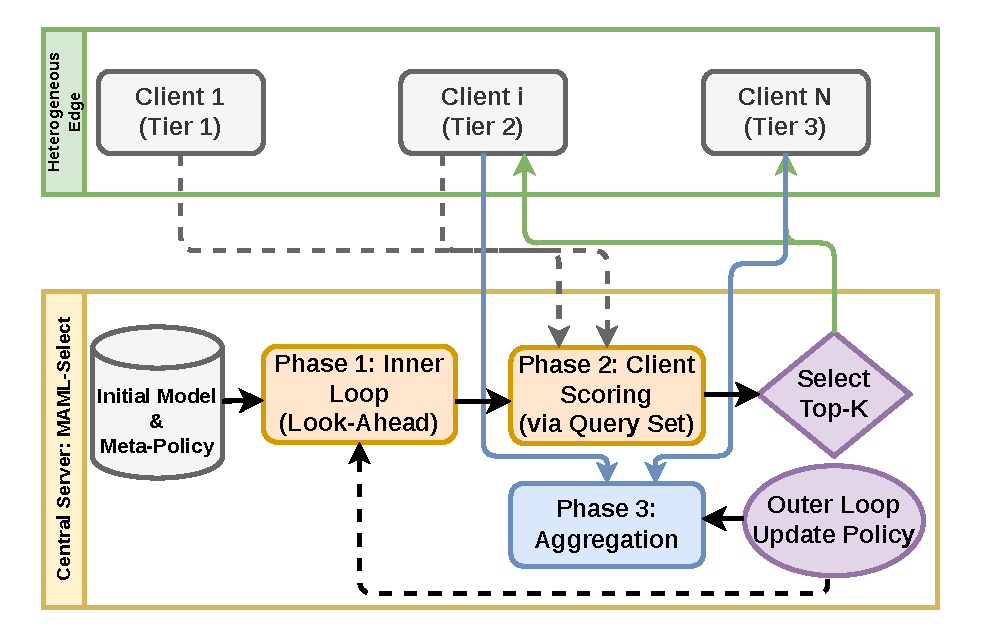
\includegraphics[width=0.62\columnwidth, trim={0.25cm 0.25cm 0.25cm 0.25cm},clip]{MAML.pdf}
\vspace{0mm}
\caption{\revision{System model and MAML-Select workflow. A central server observes client states, selects $K$ clients from the available pool, aggregates their local updates, and uses returned local-loss and system feedback for support-set adaptation, candidate scoring, and query-set meta-update.}}
\vspace{1mm}
\label{fig:model_diagram}
\end{figure}

\begin{algorithm}[!t]
	\vspace{0.5mm}
	\caption{\small MAML-Select Algorithm}
	\label{alg:maml_select}
	\begin{algorithmic}[1]
		\scriptsize
		\State \textbf{Initialize:} Global model $\theta_0$; meta-policy parameters $\phi$; inner LR $\beta$; outer LR $\eta$; trade-off $\lambda$.
		\For{round $t = 1, \ldots, T$}
		\State Server broadcasts global model $\theta_t$ to all clients.
		\State Collect state vectors $\bm{s}_{i,t}$ from available clients.
		\If{$t > 1$}
		\State \texttt{// Phase 1: Inner Loop Adaptation}
		\State Construct $\mathcal{D}_{sup}$ from round $t-1$ results.
			\State \revision{Compute fast weights $\phi'_t$ using~\eqref{eq:inner_loop}.}
		\Else
		\State $\phi'_t \leftarrow \phi_t$ \quad \texttt{// No adaptation for the first round}
		\EndIf
		\State \texttt{// Phase 2: Client Selection}
			\State \revision{Score clients: $\text{score}_i = h_{\phi'_t}(\bm{s}_{i,t})$ for all $i \in \mathcal{A}_t$.}
			\State \revision{Select lowest-cost clients: $\mathcal{S}_t \leftarrow \operatorname{Top-}K(-\text{scores})$.}
			\State \texttt{// FL Training Round}
				\State \revision{Receive local updates $\{\Delta\theta_{i,t}\}_{i \in \mathcal{S}_t}$, local losses, and system metrics.}
			\State \revision{Aggregate: $\theta_{t+1} \leftarrow \theta_t + \sum_{i \in \mathcal{S}_t} \frac{n_i}{\sum_{j \in \mathcal{S}_t}n_j}\Delta\theta_{i,t}$.}
			\State \texttt{// Phase 3: Outer Loop Meta-Update}
			\State Compute costs $c_{i,t}$ using~\eqref{eq:cost} for $i \in \revision{\mathcal{S}_t}$.
			\State Construct $\mathcal{D}_{query}(t) = \{(\bm{s}_{i,t}, c_{i,t}) \mid i \in \revision{\mathcal{S}_t}\}$.
				\State \revision{Meta-update: $\phi_{t+1} \leftarrow \phi_t - \eta \nabla_{\phi'_t} \mathcal{L}_{query}(h_{\phi'_t};\mathcal{D}_{query}(t))$.}
		\EndFor
	\end{algorithmic}
\end{algorithm}

\revision{MAML-Select differs from fixed-rule selectors because its ranking policy is adapted before each decision. It also differs from RL selectors because the update is an explicit gradient step on recent support feedback. The method is designed for rapidly changing client utility.}

\subsubsection{Computational Complexity}
\revision{Let $P=|\phi|$ denote the number of meta-policy parameters. For the $6$-$64$-$64$-$1$ MLP used here, $P=4{,}673$. A forward pass for one client costs $\mathcal{O}(P)$, so scoring $N$ available clients costs $\mathcal{O}(NP)$. Selecting the best $K$ clients can be implemented with a size-$K$ heap in $\mathcal{O}(N\log K)$, or by partial sorting. The inner support update and outer query update each use at most the selected cohort and therefore cost $\mathcal{O}(KP)$. Thus the per-round server-side selection computational cost is}
\begin{equation}
	\color{black}
	\mathcal{O}\!\left(NP + N\log K + 2KP\right).
	\label{eq:selector_complexity}
\end{equation}
\revision{Since $P$ and $K$ are fixed in the experimental protocol ($P=4{,}673$, $K=10$), MAML-Select scales linearly with the client pool size $N$. The memory cost is $\mathcal{O}(P+N+K)$ for the policy parameters, client scores, and selected cohort. This results is in contrast with correlation-matrix or Gaussian-Process selection approaches where the covariance operations can grow beyond linearly, and in common FedCor-style implementations cubically, with $N$~\cite{tang2022fedcor}.}

% =====================================================================
% V. EVALUATION AND RESULTS
% =====================================================================
\section{Evaluation and Results}

\revision{We evaluate on three benchmarks: Fashion-MNIST with LightCNN-9~\cite{wu2018light}, and CIFAR-10 and CIFAR-100 with ResNet18~\cite{he2016deep}.} \revision{$N = 100$ clients are simulated with non-IID data partition (Dirichlet $\alpha = 0.5$), selecting $K = 10$ clients per round for $T = 200$ rounds (\revision{$150$ rounds for CIFAR-100}) with $E = 5$ local epochs and batch size 32.} \revision{Table~\ref{tab:main_summary} reports mean $\pm$ standard deviation over repeated runs. The tests use seeds $42$, $123$, and $2026$.} \revision{Local models use PyTorch default initialization and stochastic gradient descent (SGD) with learning rate $0.01$, momentum $0.9$, weight decay $10^{-4}$, and a constant scheduler. The meta-policy uses one inner step with $\beta=0.01$ and Adam for the outer update with $\eta=0.001$. The selector seed is fixed to $2026$ so the reported variance reflects model-training and data-partition randomness; the simulation is fully specified by Algorithm~\ref{alg:maml_select} and the stated parameters.} \revision{Processing rates follow three device tiers that reflect the systems heterogeneity common in federated deployments~\cite{li2020federated}: Tier~1 (20\%, $1.0\times$), Tier~2 (50\%, $2.0\times$), and Tier~3 (30\%, $4.0\times$).} \revision{Resource accounting uses the same tiers: Tier~1 devices use $4$~W power and $18$~watt-hour (Wh) batteries, Tier~2 uses 7~W and 30~Wh, and Tier~3 uses 12~W and 48~Wh. Round time is straggler-bound by the slowest selected client. 
} {\color{blue}The target latency deadline $T_{target}$ is set to the average round latency of Tier~2 clients, and the trade-off parameter $\lambda = 0.5$. \revision{Baselines are FedAvg, FedCS, Oort, TiFL, FedCor, FedGCS, and CriticalFL, as characterized in Table~\ref{tab:related_work_comparison}.}}

\subsection{\revision{Accuracy and Resource Cost}}
\revision{We estimate the client-training computational cost per round as}
\begin{equation}
	\text{TFLOPs}_{total} = \sum_{t=1}^{T} \sum_{i \in \mathcal{S}_t} E\, n_i\, C_{model} \times 10^{-12},
	\label{eq:tflops}
\end{equation}
\revision{where $C_{model}$ is the same per-sample cost (FLOPs) as in $T_{i,t}^{comp}$, so the reported cost is consistent with the latency model (one ResNet18/CIFAR-10 round is $\approx4.13$ TFLOPs). Modelled energy accumulates per-tier power over local-training time:}
\begin{equation}
\color{black}
E_{total}=\sum_{t=1}^{T}\sum_{i\in\mathcal{S}_t} \frac{P_i\,T_{i,t}^{comp}}{3600},
\label{eq:energy}
\end{equation}
\revision{where $P_i$ is the device-tier power in watts and $T_{i,t}^{comp}$ is in seconds, so $E_{total}$ accumulates in watt-hours (Wh).}

\revision{Table~\ref{tab:main_summary} summarises all methods. MAML-Select attains accuracy on par with FedAvg and FedGCS on Fashion-MNIST ($90.1\%$ vs.\ $90.2\%$ and $90.7\%$) and CIFAR-100 ($58.2\%$ vs.\ $59.7\%$ and $58.7\%$). The proposed method also exceeds FedCS, Oort, TiFL, FedCor, and CriticalFL on CIFAR-100 accuracy. On CIFAR-10, a moderate accuracy reduction ($75.6\%$ vs.\ FedAvg $79.4\%$) can be observed for substantially lower computational cost. Overall, the MAML-Select offers a resource-aware operating point, staying close to the strongest accuracy baselines while reducing TFLOPs and modelled energy consumption across all reported non-IID settings. The meta-update computational overhead ($\varepsilon \approx 0.001$ GFLOPs per round) is negligible relative to client training. }

\revision{Accuracy is also tested with paired $t$-tests over the three seeds. Paired tests against FedAvg support the resource reductions on all datasets: TFLOPs $p$-values are $0.009/0.002/0.012$, and energy-consumption $p$-values are $0.007/0.001/0.003$ for Fashion-MNIST/CIFAR-10/CIFAR-100. Against FedGCS, MAML-Select is statistically indistinguishable on CIFAR-10 ($p=0.10$) and CIFAR-100 ($p=0.49$), and trails by only $0.5$~pp (percentage point) on Fashion-MNIST ($p=0.04$). Against FedAvg, the two are statistically equivalent on Fashion-MNIST ($-0.1$~pp, $p=0.84$), whereas CIFAR-10 ($-3.8$~pp, $p=0.04$) and CIFAR-100 ($-1.9$~pp, $p=0.04$) show the best energy efficiency at the expense of a negligible reduction in accuracy. For CIFAR-10, the $75.6\%$ is the converged $200$-round accuracy; the lower $\lambda$-study numbers are $100$-round diagnostics. Lowering $\lambda$ from $0.5$ to $0.1$ raises diagnostic accuracy by only about one point, so the residual gap is not mainly a $\lambda$ effect but reflects the harder ResNet18 task, where one low-cost cohort per round can miss useful class variation. We therefore interpret the CIFAR-10 result as an efficiency-oriented operating point, where MAML-Select prioritizes lower resource use over peak final accuracy.}

\begin{table*}[!t]
\centering
\color{blue}
\caption{Benchmark summary across non-IID datasets. Accuracy, precision, recall, F1, and coverage are in percent; energy is in Watt-hour (Wh).}
\label{tab:main_summary}
\begingroup
\scriptsize
\setlength{\tabcolsep}{2.4pt}
\renewcommand{\arraystretch}{0.96}
\begin{tabular*}{\textwidth}{@{\extracolsep{\fill}}lcccccccc@{}}
\toprule
Method & Acc. & Prec. & Rec. & F1 & TFLOPs & Energy & Jain & Cov. \\
\midrule
\multicolumn{9}{@{}l}{\textit{Fashion-MNIST}} \\
FedAvg        & 90.22$\pm$0.58 & 90.55$\pm$0.20 & 90.22$\pm$0.58 & 90.22$\pm$0.51 & 140$\pm$1       & 5752$\pm$72     & 0.95$\pm$0.00 & 100$\pm$0 \\
FedCS         & 84.11$\pm$1.82 & 84.84$\pm$0.77 & 84.11$\pm$1.82 & 83.91$\pm$1.98 & 76$\pm$7        & 2772$\pm$211    & 0.10$\pm$0.00 & 10$\pm$0  \\
Oort          & 86.70$\pm$0.19 & 86.66$\pm$0.21 & 86.70$\pm$0.19 & 86.42$\pm$0.26 & 149$\pm$8       & 5963$\pm$456    & 0.10$\pm$0.00 & 10$\pm$0  \\
TiFL          & 86.73$\pm$0.34 & 86.62$\pm$0.26 & 86.73$\pm$0.34 & 86.51$\pm$0.34 & 147$\pm$6       & 6062$\pm$348    & 0.11$\pm$0.00 & 12$\pm$0  \\
FedCor        & 89.35$\pm$0.50 & 89.31$\pm$0.51 & 89.35$\pm$0.50 & 89.22$\pm$0.57 & 121$\pm$5       & 4845$\pm$204    & 0.26$\pm$0.04 & 49$\pm$8  \\
CriticalFL    & 90.16$\pm$0.47 & 90.24$\pm$0.38 & 90.17$\pm$0.47 & 90.11$\pm$0.42 & 304$\pm$143     & 12552$\pm$5860  & 0.98$\pm$0.01 & 100$\pm$0 \\
FedGCS        & 90.65$\pm$0.29 & 90.73$\pm$0.16 & 90.65$\pm$0.29 & 90.63$\pm$0.26 & 136$\pm$4       & 5595$\pm$113    & 0.95$\pm$0.02 & 100$\pm$0 \\
\textbf{MAML-Select} & \textbf{90.11$\pm$0.47} & \textbf{90.43$\pm$0.04} & \textbf{90.11$\pm$0.47} & \textbf{90.04$\pm$0.30} & \textbf{122$\pm$2} & \textbf{4809$\pm$79} & \textbf{0.77$\pm$0.06} & \textbf{100$\pm$0} \\
\midrule
\multicolumn{9}{@{}l}{\textit{CIFAR-10}} \\
FedAvg        & 79.43$\pm$1.84 & 80.01$\pm$1.28 & 79.43$\pm$1.84 & 79.36$\pm$1.78 & 8341$\pm$52     & 4798$\pm$24     & 0.95$\pm$0.00 & 100$\pm$0 \\
FedCS         & 50.45$\pm$2.57 & 50.88$\pm$2.60 & 50.45$\pm$2.57 & 49.87$\pm$2.33 & 4081$\pm$600    & 2073$\pm$262    & 0.10$\pm$0.00 & 10$\pm$0  \\
Oort          & 60.19$\pm$5.18 & 60.84$\pm$4.97 & 60.19$\pm$5.18 & 59.69$\pm$4.61 & 8303$\pm$1923   & 4677$\pm$856    & 0.10$\pm$0.00 & 10$\pm$0  \\
TiFL          & 61.93$\pm$5.04 & 62.48$\pm$4.78 & 61.93$\pm$5.04 & 61.36$\pm$4.60 & 8200$\pm$2143   & 4800$\pm$1203   & 0.11$\pm$0.00 & 12$\pm$0  \\
FedCor        & 67.20$\pm$5.33 & 67.83$\pm$4.74 & 67.20$\pm$5.33 & 66.81$\pm$5.37 & 7748$\pm$695    & 4452$\pm$435    & 0.20$\pm$0.02 & 31$\pm$5  \\
CriticalFL    & 77.34$\pm$5.21 & 79.98$\pm$2.80 & 77.34$\pm$5.21 & 77.46$\pm$5.21 & 14239$\pm$4864  & 8205$\pm$2807   & 0.98$\pm$0.01 & 100$\pm$0 \\
FedGCS        & 77.88$\pm$1.75 & 78.93$\pm$1.50 & 77.88$\pm$1.75 & 77.69$\pm$1.54 & 7656$\pm$278    & 4428$\pm$154    & 0.90$\pm$0.03 & 100$\pm$0 \\
\textbf{MAML-Select} & \textbf{75.63$\pm$1.43} & \textbf{76.51$\pm$1.55} & \textbf{75.63$\pm$1.43} & \textbf{75.25$\pm$1.34} & \textbf{6549$\pm$118} & \textbf{3610$\pm$60} & \textbf{0.61$\pm$0.01} & \textbf{100$\pm$0} \\
\midrule
\multicolumn{9}{@{}l}{\textit{CIFAR-100}} \\
FedAvg        & 59.66$\pm$0.29 & 60.90$\pm$0.48 & 59.66$\pm$0.29 & 59.13$\pm$0.40 & 6331$\pm$6      & 3626$\pm$18     & 0.94$\pm$0.00 & 100$\pm$0 \\
FedCS         & 27.52$\pm$0.29 & 27.93$\pm$0.10 & 27.52$\pm$0.29 & 26.39$\pm$0.09 & 5334$\pm$23     & 2659$\pm$12     & 0.10$\pm$0.00 & 10$\pm$0  \\
Oort          & 29.41$\pm$1.73 & 29.82$\pm$1.77 & 29.41$\pm$1.73 & 28.13$\pm$1.73 & 5955$\pm$189    & 3421$\pm$181    & 0.10$\pm$0.00 & 10$\pm$0  \\
TiFL          & 32.12$\pm$0.30 & 33.07$\pm$0.50 & 32.12$\pm$0.33 & 31.02$\pm$0.42 & 5986$\pm$28     & 3499$\pm$14     & 0.11$\pm$0.00 & 12$\pm$0  \\
FedCor        & 34.18$\pm$0.24 & 33.89$\pm$0.26 & 34.18$\pm$0.60 & 32.93$\pm$0.20 & 6428$\pm$32     & 3668$\pm$18     & 0.12$\pm$0.00 & 14$\pm$0  \\
CriticalFL    & 48.84$\pm$1.58 & 60.56$\pm$1.89 & 48.84$\pm$1.58 & 48.07$\pm$2.32 & 9469$\pm$392    & 5438$\pm$214    & 0.97$\pm$0.00 & 100$\pm$0 \\
FedGCS        & 58.66$\pm$0.11 & 60.24$\pm$0.03 & 58.66$\pm$0.11 & 58.08$\pm$0.20 & 6140$\pm$24     & 3526$\pm$4      & 0.82$\pm$0.02 & 100$\pm$0 \\
\textbf{MAML-Select} & \textbf{58.15$\pm$0.51} & \textbf{59.87$\pm$0.55} & \textbf{58.15$\pm$0.51} & \textbf{57.66$\pm$0.33} & \textbf{6224$\pm$20} & \textbf{3457$\pm$6} & \textbf{0.78$\pm$0.03} & \textbf{100$\pm$0} \\
\bottomrule
\end{tabular*}
\endgroup
\end{table*} 
\revision{Fig.~\ref{fig:convergence} summarises the CIFAR-100 behaviour. MAML-Select remains close to FedAvg and FedGCS on accuracy and loss while staying in the low energy-consumption cluster, and panel~(b) shows the selector meta-update settling.}

\begin{figure}[!tb]
\centering

\includegraphics[width=\columnwidth]{fig_convergence_boxed.pdf}
\caption{\revision{CIFAR-100 convergence over 150 rounds. The panels report (a)~accuracy, (b)~the selector meta-update magnitude $\lVert\phi_{t+1}-\phi_t\rVert_2$ for MAML-Select (the empirical signature of Corollary~\ref{cor:rate}), (c)~cumulative modelled energy consumption, and (d)~test loss.}}
\label{fig:convergence}
\end{figure}

\revision{Fig.~\ref{fig:effscale}(a) shows the efficiency--accuracy trade-off: MAML-Select is consistently in the lower-computational-cost region while staying close to the strongest baselines in accuracy. Relative to FedAvg over shared seeds, it lowers cumulative TFLOPs by $12.8\%$/$21.5\%$/$1.7\%$ and modelled energy consumption by $16.4\%$/$24.7\%$/$4.7\%$ on Fashion-MNIST/CIFAR-10/CIFAR-100, for accuracy changes of $-0.1$/$-3.8$/$-1.5$ percentage points. The main empirical gain is thus resource efficiency with competitive accuracy: the selector keeps broad data coverage while operating at a lower computational-cost point than several utility-driven alternatives.}

\begin{figure}[!tb]
\centering
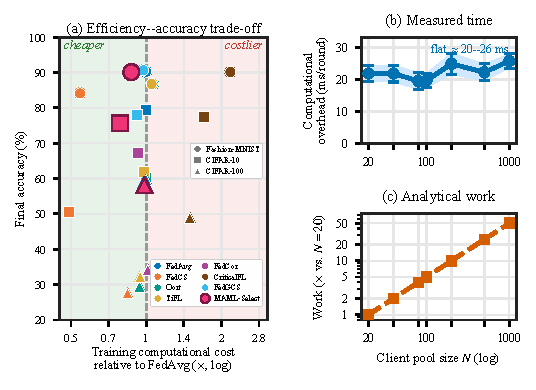
\includegraphics[width=\columnwidth]{fig_efficiency_scaling_boxed.pdf}
\caption{\revision{(a)~Efficiency--accuracy trade-off: the $x$-axis is cumulative training computational cost relative to FedAvg (log scale; $x<1$ is cheaper than FedAvg), the $y$-axis is final accuracy, and marker shape encodes the dataset. (b)~Measured per-round selection computational overhead (mean with $95\%$ confidence intervals over $10$ rounds) and (c)~the analytical operation count $C(N,K)=NP+N\log K+2KP$ from~\eqref{eq:selector_complexity} (policy size $P=4{,}673$, normalized to its value at $N=20$), both as the client pool size $N$ grows with the selection rate held at $10\%$ ($K/N=0.1$).}}
\label{fig:effscale}
\end{figure}

\revision{We measure participation fairness with Jain's index on the per-client selection counts $\{p_i\}_{i=1}^{N}$, defined as $J=\big(\sum_{i} p_i\big)^2 / \big(N\sum_{i} p_i^2\big)$, which lies in $[1/N,1]$ with $J=1$ for perfectly even selection and smaller values for more concentrated selection. We also report participation coverage, the percentage of clients selected at least once, $\mathrm{Cov}=\tfrac{100}{N}\,\big|\{\,i:\sum_{t=1}^{T} a_{i,t}\ge 1\,\}\big|$, where $\mathrm{Cov}=100\%$ means no client is ever permanently excluded. MAML-Select reaches $100\%$ client coverage on every dataset. While its Jain index ($0.61$--$0.78$) is lower than FedAvg and FedGCS, perfect coverage demonstrates that the policy does not permanently exclude any clients.}

\subsection{\revision{Selector Scaling}}
\revision{To validate the complexity expression in~\eqref{eq:selector_complexity}, we measured the server-side selection computational overhead of MAML-Select over 10 rounds. We varied the client pool size as $N\in\{20,40,80,100,200,500,1000\}$ and held the selection rate fixed at $10\%$ ($K/N=0.1$). Fig.~\ref{fig:effscale}(b) shows that the measured computational overhead stays nearly flat, between approximately $20$ and $26$ ms per round, even as $N$ grows fifty-fold to $1000$.
%The analytical cost is $NP + N\log K + 2KP$, where $P=4{,}673$ is the number of policy parameters.
With the selection rate held at $10\%$, the $\mathcal{O}(NP)$ scoring term dominates, so the operation count grows about linearly with $N$ (Fig.~\ref{fig:effscale}(c)). The measured time stays flat because at these sizes the small $\mathcal{O}(NP)$ scoring cost is dominated by fixed per-round bookkeeping, so the selector is inexpensive even at $N=1000$. The one-step inner loop is used intentionally. Additional inner steps increase the adaptation cost, while the ablation results show that one step gives the best accuracy with the lowest overhead.}

\subsection{\revision{Sensitivity and Ablation}}
\revision{These experiments test whether MAML-Select is stable when its design choices are perturbed. We probe four choices: the cost trade-off $\lambda$, the number of inner-loop steps, the selector width, and the six-feature policy state. To keep the diagnostic budget tractable, each ablation is reported on the dataset where it is most informative.}

\revision{Fig.~\ref{fig:lambda_sensitivity} reports the $\lambda$ sweep on both Fashion-MNIST and CIFAR-10. A larger $\lambda$ gives more weight to lower utility clients, so computational cost and energy consumption fall on both datasets. On Fashion-MNIST, accuracy stays nearly flat, within about one point. On CIFAR-10, the trade-off is sharper: accuracy drops from $64.9\%$ at $\lambda=0.1$ to $56.3\%$ at $\lambda=5$, while computational cost falls by about $26\%$ and energy consumption by about $30\%$. Fairness also falls at large $\lambda$. We keep $\lambda=0.5$ as the default. It stays close to the best accuracy, lowers cost, and avoids the sharp fairness loss seen at $\lambda\ge1$.}

\begin{figure}[!tb]
\centering

\includegraphics[width=\columnwidth]{fig_lambda_two_dataset_boxed.pdf}
\caption{\revision{Sensitivity to the cost trade-off $\lambda$ on Fashion-MNIST (left) and CIFAR-10 (right). The black curve is accuracy. Computational cost, energy consumption, and fairness are normalized to their $\lambda=0.1$ values. The trade-off is mild on Fashion-MNIST and sharper on CIFAR-10.}}
\label{fig:lambda_sensitivity}
\end{figure}

\revision{Table~\ref{tab:design_ablation} depicts the choices of two ablations. On CIFAR-10, a single inner step gives the highest accuracy ($63.8\%$) and the lowest overhead ($38.7$ versus $45.2$~ms at five steps), so we use one step. On Fashion-MNIST, accuracy stays within about $0.6$ points as the width grows over $h\in\{16,32,64,128\}$ ($401$ to $17{,}537$ parameters), so the compact $h=64$ default is robust.}

\begin{table}[H]
\centering
\color{blue}
\caption{\revision{Inner-step (CIFAR-10) and selector-width (Fashion-MNIST) ablations: final accuracy and selection computational overhead, mean$\pm$std over three seeds. Defaults ($1$ step, $h=64$) in bold.}}
\label{tab:design_ablation}
\scriptsize
\setlength{\tabcolsep}{4pt}
\renewcommand{\arraystretch}{0.92}
\begin{tabular*}{\columnwidth}{@{\extracolsep{\fill}}llrr@{}}
\toprule
\revision{Ablation} & \revision{Setting} & \revision{Acc.\ (\%)} & \revision{\shortstack[r]{Computational\\ overhead (ms)}} \\
\midrule
\revision{Inner steps} & \revision{\textbf{1}} & \revision{63.8$\pm$1.8} & \revision{38.7} \\
 & \revision{2} & \revision{63.1$\pm$1.8} & \revision{39.8} \\
 & \revision{5} & \revision{62.2$\pm$2.4} & \revision{45.2} \\
\addlinespace[1pt]
\revision{Width $h$} & \revision{16} & \revision{90.0$\pm$0.3} & \revision{10.2} \\
 & \revision{32} & \revision{90.6$\pm$0.3} & \revision{10.4} \\
 & \revision{\textbf{64}} & \revision{90.1$\pm$0.5} & \revision{10.2} \\
 & \revision{128} & \revision{90.3$\pm$0.7} & \revision{11.6} \\
\bottomrule
\end{tabular*}
\end{table}

\revision{Table~\ref{tab:ablation} removes one state feature at a time (Fashion-MNIST). Accuracy changes stay within about $0.35$ points, so the policy is robust to any single removal. The largest drop comes from the battery feature ($-0.33$~pp), with latency and loss also contributing; removing the frequency feature raises accuracy slightly but lowers the Jain index the most ($0.78\!\to\!0.65$), so the participation features chiefly protect fairness. These results support the full six-feature state because it preserves both accuracy stability and participation balance.}

\begin{table}[H]
\centering
\color{blue}
\caption{State-feature ablation on Fashion-MNIST ($n=3$); each row removes one feature from the six-dimensional state vector.}
\label{tab:ablation}
\scriptsize
\setlength{\tabcolsep}{3.4pt}
\renewcommand{\arraystretch}{0.92}
\begin{tabular*}{\columnwidth}{@{\extracolsep{\fill}}lrrr@{}}
\toprule
Variant & Acc.\ (\%) & TFLOPs & Jain \\
\midrule
\textbf{Full state vector} & 90.23\,$\pm$\,0.55 & 122 & 0.78 \\
w/o loss & 90.16\,$\pm$\,0.66 & 123 & 0.79 \\
w/o gradient norm & 90.30\,$\pm$\,0.24 & 122 & 0.78 \\
w/o latency & 90.14\,$\pm$\,0.14 & 119 & 0.70 \\
w/o battery & 89.90\,$\pm$\,0.44 & 122 & 0.79 \\
w/o frequency & 90.47\,$\pm$\,0.13 & 115 & 0.65 \\
w/o staleness & 90.37\,$\pm$\,0.19 & 123 & 0.78 \\
\bottomrule
\end{tabular*}
\vspace{0mm}
\end{table}


% =====================================================================
% VI. CONCLUSION
% =====================================================================
\FloatBarrier
\section{Conclusion and Future Work}
\revision{We introduced MAML-Select, an online adaptive client-selection framework for heterogeneous FL that learns a lightweight ranking policy over both learning feedback and system-state information, adapting it with recent support-set feedback before each selection decision.
Across Fashion-MNIST, CIFAR-10, and CIFAR-100, MAML-Select achieves competitive accuracy while reducing cumulative computational cost and modelled energy consumption compared with higher-cost selection strategies. The $\lambda$-sensitivity study shows that the cost trade-off can be tuned without destabilizing accuracy, and the ablations confirm that a single inner step, a compact policy network, and the full six-feature state are sufficient for stable selection. Future work will broaden the evaluation across heterogeneity levels, client-pool sizes, and naturally federated benchmarks, and will study an asynchronous extension that relaxes the synchronous-round assumption together with a differentially private treatment of the client-state vector so that selection does not leak device information.}

\balance
%=====================================================================
% REFERENCES
% =====================================================================
\vspace{-1mm}
% Tighten inter-reference spacing to keep the bibliography compact.
\let\OLDthebibliography\thebibliography
\renewcommand\thebibliography[1]{%
  \OLDthebibliography{#1}%
  \setlength{\itemsep}{0pt plus 0.2pt}%
  \setlength{\parsep}{0pt}%
  \setlength{\topsep}{0pt}}
{\scriptsize
\begin{thebibliography}{10}
\providecommand{\url}[1]{#1}
\csname url@samestyle\endcsname
\providecommand{\newblock}{\relax}
\providecommand{\bibinfo}[2]{#2}
\providecommand{\BIBentrySTDinterwordspacing}{\spaceskip=0pt\relax}
\providecommand{\BIBentryALTinterwordstretchfactor}{4}
\providecommand{\BIBentryALTinterwordspacing}{\spaceskip=\fontdimen2\font plus
\BIBentryALTinterwordstretchfactor\fontdimen3\font minus \fontdimen4\font\relax}
\providecommand{\BIBforeignlanguage}[2]{{%
\expandafter\ifx\csname l@#1\endcsname\relax
\typeout{** WARNING: IEEEtran.bst: No hyphenation pattern has been}%
\typeout{** loaded for the language `#1'. Using the pattern for}%
\typeout{** the default language instead.}%
\else
\language=\csname l@#1\endcsname
\fi
#2}}
\providecommand{\BIBdecl}{\relax}
\BIBdecl

\bibitem{mcmahan2017communication}
B.~McMahan, E.~Moore, D.~Ramage, S.~Hampson, and B.~Ag{\"u}era~y Arcas, ``Communication-efficient learning of deep networks from decentralized data,'' in \emph{Artificial Intelligence and Statistics}.\hskip 1em plus 0.5em minus 0.4em\relax PMLR, 2017, pp. 1273--1282.

\bibitem{karimireddy2020scaffold}
S.~P. Karimireddy, S.~Kale, M.~Mohri, S.~Reddi, S.~Stich, and A.~T. Suresh, ``{SCAFFOLD}: Stochastic controlled averaging for federated learning,'' in \emph{International Conference on Machine Learning}.\hskip 1em plus 0.5em minus 0.4em\relax PMLR, 2020, pp. 5132--5143.

\bibitem{mai2024study}
V.~S. Mai, R.~J. La, and T.~Zhang, ``A study of enhancing federated learning on non-{IID} data with server learning,'' \emph{IEEE Transactions on Artificial Intelligence}, vol.~5, no.~11, pp. 5589--5604, 2024.

\bibitem{tapwal2026stragglers}
\revision{R.~Tapwal, ``Stragglers reimagined: Explainability-driven adaptive federated learning for resource constrained {IoMT} system,'' \emph{IEEE Transactions on Artificial Intelligence}, vol.~7, no.~2, pp. 1002--1011, 2026.}

\bibitem{forootani2026asynchronous}
\revision{A.~Forootani and R.~Iervolino, ``Asynchronous federated learning with nonconvex client objective functions and heterogeneous dataset,'' \emph{IEEE Transactions on Artificial Intelligence}, vol.~7, no.~5, pp. 2610--2624, 2026.}

\bibitem{borazjani2026redefining}
\revision{K.~Borazjani, P.~Abdisarabshali, N.~Khosravan, and S.~Hosseinalipour, ``Redefining non-{IID} data in federated learning for computer vision tasks: Migrating from labels to embeddings for task-specific data distributions,'' \emph{IEEE Transactions on Artificial Intelligence}, 2026, early Access.}

\bibitem{nishio2019client}
T.~Nishio and R.~Yonetani, ``Client selection for federated learning with heterogeneous resources in mobile edge,'' in \emph{IEEE International Conference on Communications (ICC)}.\hskip 1em plus 0.5em minus 0.4em\relax IEEE, 2019, pp. 1--7.

\bibitem{chai2020tifl}
Z.~Chai, A.~Ali, S.~Zawad, S.~Truex, A.~Anwar, N.~Baracaldo, Y.~Zhou, H.~Ludwig, F.~Yan, and Y.~Cheng, ``{TiFL}: A tier-based federated learning system,'' in \emph{Proceedings of the 29th International Symposium on High-Performance Parallel and Distributed Computing}, 2020, pp. 125--136.

\bibitem{lai2021oort}
F.~Lai, X.~Zhu, H.~V. Madhyastha, and M.~Chowdhury, ``{Oort}: Efficient federated learning via guided participant selection,'' in \emph{15th USENIX Symposium on Operating Systems Design and Implementation}, 2021, pp. 19--35.

\bibitem{tang2022fedcor}
M.~Tang, X.~Ning, Y.~Wang, J.~Sun, Y.~Wang, H.~Li, and Y.~Chen, ``{FedCor}: Correlation-based active client selection strategy for heterogeneous federated learning,'' in \emph{IEEE/CVF Conference on Computer Vision and Pattern Recognition}.\hskip 1em plus 0.5em minus 0.4em\relax IEEE, 2022, pp. 10\,102--10\,111.

\bibitem{xu2024federated}
Y.~Xu, Z.~Jiang, H.~Xu, Z.~Wang, C.~Qian, and C.~Qiao, ``Federated learning with client selection and gradient compression in heterogeneous edge systems,'' \emph{IEEE Transactions on Mobile Computing}, vol.~23, no.~5, pp. 5446--5461, 2024.

\bibitem{yan2023criticalfl}
G.~Yan, H.~Wang, X.~Yuan, and J.~Li, ``{CriticalFL}: A critical learning periods augmented client selection framework for efficient federated learning,'' in \emph{Proceedings of the 29th ACM SIGKDD Conference on Knowledge Discovery and Data Mining}, 2023, pp. 5034--5044.

\bibitem{ning2024fedgcs}
Z.~Ning, C.~Tian, M.~Xiao, W.~Fan, P.~Wang, L.~Li, P.~Wang, and Y.~Zhou, ``{FedGCS}: A generative framework for efficient client selection in federated learning via gradient-based optimization,'' in \emph{Proceedings of the 33rd International Joint Conference on Artificial Intelligence}, 2024, pp. 4760--4768.

\bibitem{wang2020optimizing}
H.~Wang, Z.~Kaplan, D.~Niu, and B.~Li, ``Optimizing federated learning on non-{IID} data with reinforcement learning,'' in \emph{IEEE INFOCOM}.\hskip 1em plus 0.5em minus 0.4em\relax IEEE, 2020, pp. 1698--1707.

\bibitem{pan2024contextual}
Q.~Pan, H.~Cao, Y.~Zhu, J.~Liu, and B.~Li, ``Contextual client selection for efficient federated learning over edge devices,'' \emph{IEEE Transactions on Mobile Computing}, vol.~23, no.~6, pp. 6538--6548, 2024.

\bibitem{kazemi2026robust}
\revision{K.~Kazemi, M.~H. Badiei, and H.~Kebriaei, ``Robust peer-to-peer federated learning with deep reinforcement learning based client selection against data poisoning attacks,'' \emph{IEEE Transactions on Artificial Intelligence}, vol.~7, no.~1, pp. 262--271, 2026.}

\bibitem{finn2017model}
C.~Finn, P.~Abbeel, and S.~Levine, ``Model-agnostic meta-learning for fast adaptation of deep networks,'' in \emph{International Conference on Machine Learning (ICML)}.\hskip 1em plus 0.5em minus 0.4em\relax PMLR, 2017, pp. 1126--1135.

\bibitem{fallah2020personalized}
A.~Fallah, A.~Mokhtari, and A.~Ozdaglar, ``Personalized federated learning with theoretical guarantees: A model-agnostic meta-learning approach,'' \emph{Advances in Neural Information Processing Systems}, vol.~33, pp. 3557--3568, 2020.

\bibitem{tran2026fedimp}
\revision{H.~A. Tran, C.~Ta, and T.~X. Tran, ``{FedImp}: Enhancing federated learning convergence with impurity-based weighting,'' \emph{IEEE Transactions on Artificial Intelligence}, vol.~7, no.~3, pp. 1652--1665, 2026.}

\bibitem{arisdakessian2026vox}
\revision{S.~Arisdakessian, O.~A. Wahab, A.~Mourad, and H.~Otrok, ``Towards vox populi in federated learning: A fair and inclusive client selection framework,'' \emph{IEEE Transactions on Artificial Intelligence}, vol.~7, pp. 1997--2011, 2026.}

\bibitem{wu2018light}
X.~Wu, R.~He, Z.~Sun, and T.~Tan, ``A light {CNN} for deep face representation with noisy labels,'' \emph{IEEE Transactions on Information Forensics and Security}, vol.~13, no.~11, pp. 2884--2896, 2018.

\bibitem{he2016deep}
K.~He, X.~Zhang, S.~Ren, and J.~Sun, ``Deep residual learning for image recognition,'' in \emph{IEEE Conference on Computer Vision and Pattern Recognition}.\hskip 1em plus 0.5em minus 0.4em\relax IEEE, 2016, pp. 770--778.

\bibitem{li2020federated}
T.~Li, A.~K. Sahu, A.~Talwalkar, and V.~Smith, ``Federated learning: Challenges, methods, and future directions,'' \emph{IEEE Signal Processing Magazine}, vol.~37, no.~3, pp. 50--60, 2020.


\end{thebibliography}
}

\end{document}
